% Adjust these for the path of the theme and its graphics, relative to this file
%\usepackage{beamerthemeFalmouthGamesAcademy}
\usepackage{../../beamerthemeFalmouthGamesAcademy}
\usepackage{multimedia}
\graphicspath{ {../../} }

% Default language for code listings
\lstset{language=C++,
        morekeywords={each,in,nullptr}
}

% For strikethrough effect
\usepackage[normalem]{ulem}
\usepackage{wasysym}

% https://tex.stackexchange.com/a/42620
\usepackage{pifont}% http://ctan.org/pkg/pifont
\newcommand{\cmark}{\ding{51}}%
\newcommand{\xmark}{\ding{55}}%


\usepackage{pdfpages}

% http://www.texample.net/tikz/examples/state-machine/
\usetikzlibrary{arrows,automata}

\newcommand{\modulecode}{COMP702}\newcommand{\moduletitle}{Classical Artificial Intelligence}\newcommand{\sessionnumber}{1}

\hypersetup{
pdftex,
pdftitle=\sessionnumber: What Is AI?,
pdfauthor=Ed Powley,
pdfdisplaydoctitle,
pdflang=en-GB
}

\begin{document}
\title{\sessionnumber: What Is AI?}
\subtitle{\modulecode: \moduletitle}

\frame{\titlepage} 

\part{What is ``Classical'' AI?}
\frame{\partpage}

\begin{frame}{What is AI?}
    \begin{itemize}
        \pause\item[\xmark] Simulating human brains or human intelligence
        \pause\item[\cmark] Performing tasks by machine (or by software) which would ordinarily require human intelligence
        \pause\item[\cmark] Making decisions to achieve goals
    \end{itemize}
\end{frame}

\begin{frame}{What is AI?}
    \begin{itemize}
        \pause\item[\xmark] Programming machines to learn by themselves
        \pause\item[\cmark] Machine learning is an important sub-field of AI, but there are many other AI techniques
    \end{itemize}
\end{frame}

\begin{frame}{What is AI?}
    \begin{itemize}
        \pause\item[\xmark] Programming machines to possess general intelligence, self-awareness, consciousness
        \pause\item[\cmark] Maybe one day, but for now this is pure sci-fi
        \pause\item[\cmark] Programming machines to carry out (or learn to carry out) a specific type of task
    \end{itemize}
\end{frame}

\begin{frame}{What is classical AI?}
    \begin{itemize}
        \pause\item A.k.a. \textbf{Good Old Fashioned AI}
        \pause\item A.k.a. \textbf{Symbolic AI}
        \pause\item Based on symbolic (``human-readable'') representations of problems, logical systems, search spaces
        \pause\item As opposed to machine learning, evolutionary algorithms etc which tend to be ``black boxes''
    \end{itemize}
\end{frame}

\begin{frame}{Applications of AI in games}
	\begin{itemize}
		\pause\item Enemies and other NPCs
		\pause\item Opponents in $\{$board, card, strategy$\}$ games
		\pause\item Automated playtesting
		\pause\item Directors, hints, adaptive difficulty
		\pause\item Procedural content generation
		\pause\item Content production tools
		\pause\item Procedural narrative
		\pause\item Agent-based simulations
		\pause\item ...
	\end{itemize}
\end{frame}

\begin{frame}{Why game AI?}
	\begin{itemize}
		\pause\item Games are a useful testbed for new AI technologies
		\pause\item Game theory is a useful mathematical abstraction for many types of problem
		\pause\item Game AI is more than pure problem solving --- game AI needs to create an entertaining experience
	\end{itemize}
\end{frame}

\part{AI architectures}
\frame{\partpage}

\begin{frame}{Rule-based AI}
	\begin{itemize}
		\pause\item Generally implemented as \texttt{if} statements or event-based triggers
		\pause\item Triggers can be complicated e.g.\ based on raycasts
	\end{itemize}
\end{frame}

\begin{frame}{Finite state machines}
	\begin{center}
		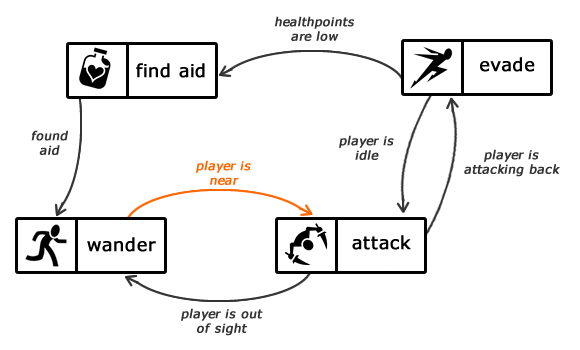
\includegraphics[width=\textwidth]{fsm_enemy_brain}
		% https://gamedevelopment.tutsplus.com/tutorials/finite-state-machines-theory-and-implementation--gamedev-11867
	\end{center}
\end{frame}

\begin{frame}{Behaviour trees}
	\begin{center}
		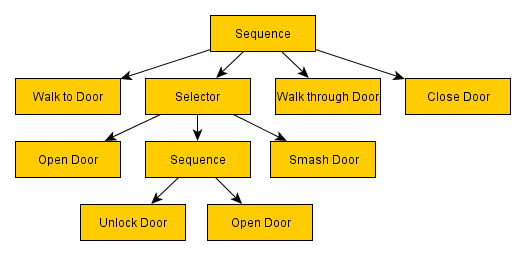
\includegraphics[width=\textwidth]{behaviour_tree}
		% https://www.gamasutra.com/blogs/ChrisSimpson/20140717/221339/Behavior_trees_for_AI_How_they_work.php
	\end{center}
\end{frame}

\begin{frame}{Multi-agent approaches (e.g.\ flocking)}
	\begin{center}
		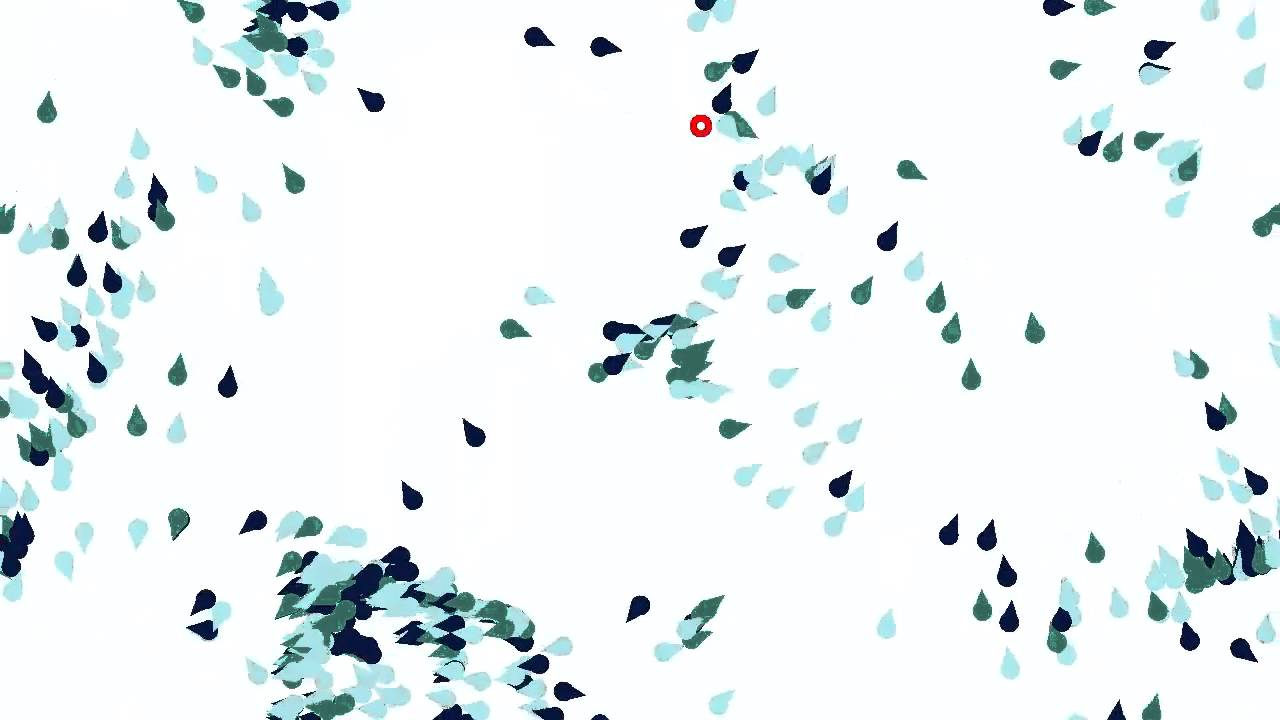
\includegraphics[width=\textwidth]{flocking}
		% https://www.youtube.com/watch?v=5p6OAEVKw-0
	\end{center}
\end{frame}

\begin{frame}{Game tree search}
	\begin{center}
		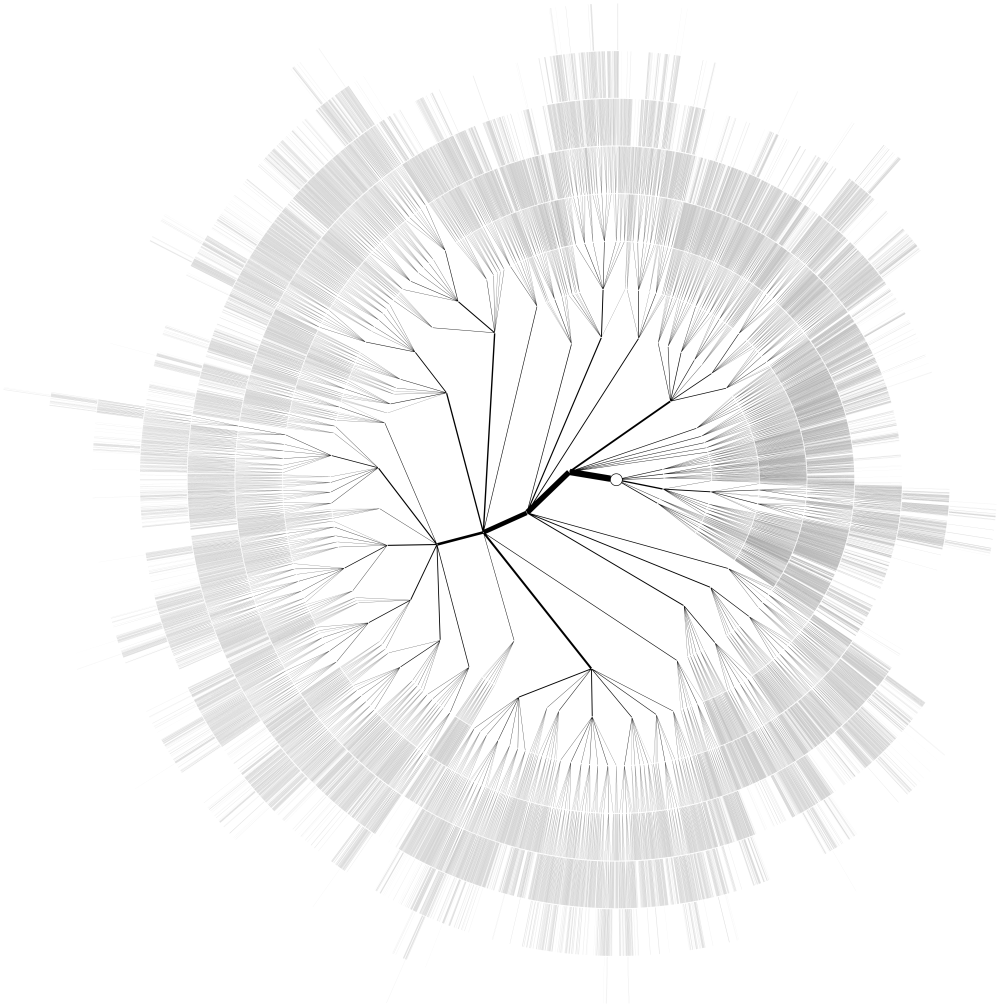
\includegraphics[height=0.7\textheight]{mcts}
	\end{center}
\end{frame}

\begin{frame}{Planning}
	\begin{center}
		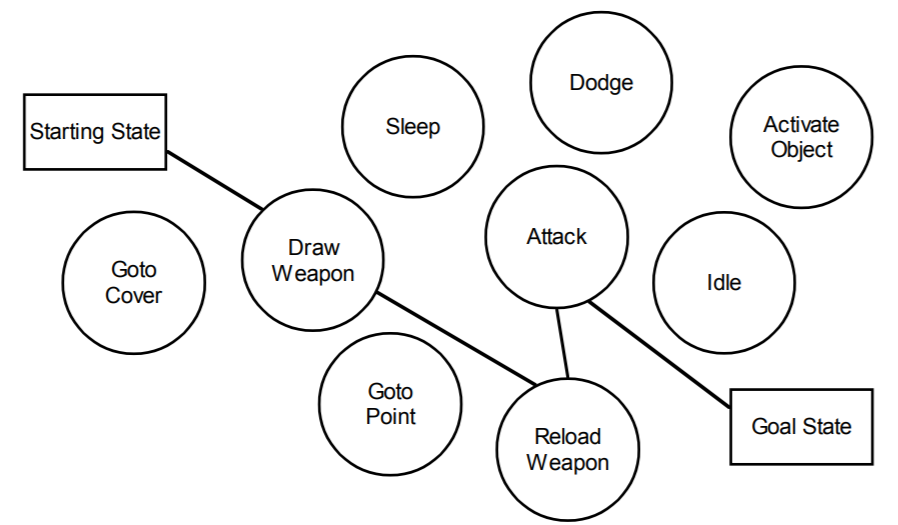
\includegraphics[width=\textwidth]{goap}
		% http://alumni.media.mit.edu/~jorkin/GOAP_draft_AIWisdom2_2003.pdf
	\end{center}
\end{frame}

\begin{frame}{Machine learning}
	\begin{center}
		\colorbox{white}{
			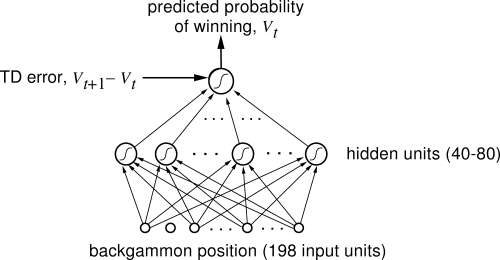
\includegraphics[width=0.7\textwidth]{tdgammon}
		}
		% https://users.auth.gr/kehagiat/Research/GameTheory/12CombBiblio/BackGammon.html
	\end{center}
\end{frame}

\begin{frame}{AI architectures}
	\begin{itemize}
		\pause\item Can roughly be divided into \textbf{hand-authored}...
			\begin{itemize}
				\pause\item Rule-based, FSM, behaviour trees
			\end{itemize}
		\pause\item ... and \textbf{computational intelligence}
			\begin{itemize}
				\pause\item Search, planning, machine learning
			\end{itemize}
		\pause\item Do you want to \textbf{design} the AI behaviours yourself,
			or do you want them to \textbf{emerge} from the system?
		\pause\item Predictability and authorial control versus adaptability and novelty
		\pause\item Can also combine the two, e.g.\ use a rule-based system to constrain a CI system
	\end{itemize}
\end{frame}


\end{document}
